\section{Event and Particle Reconstruction}

\begin{frame}
    \centering
    \frametitle{Event and Particle Reconstruction}
\begin{figure}
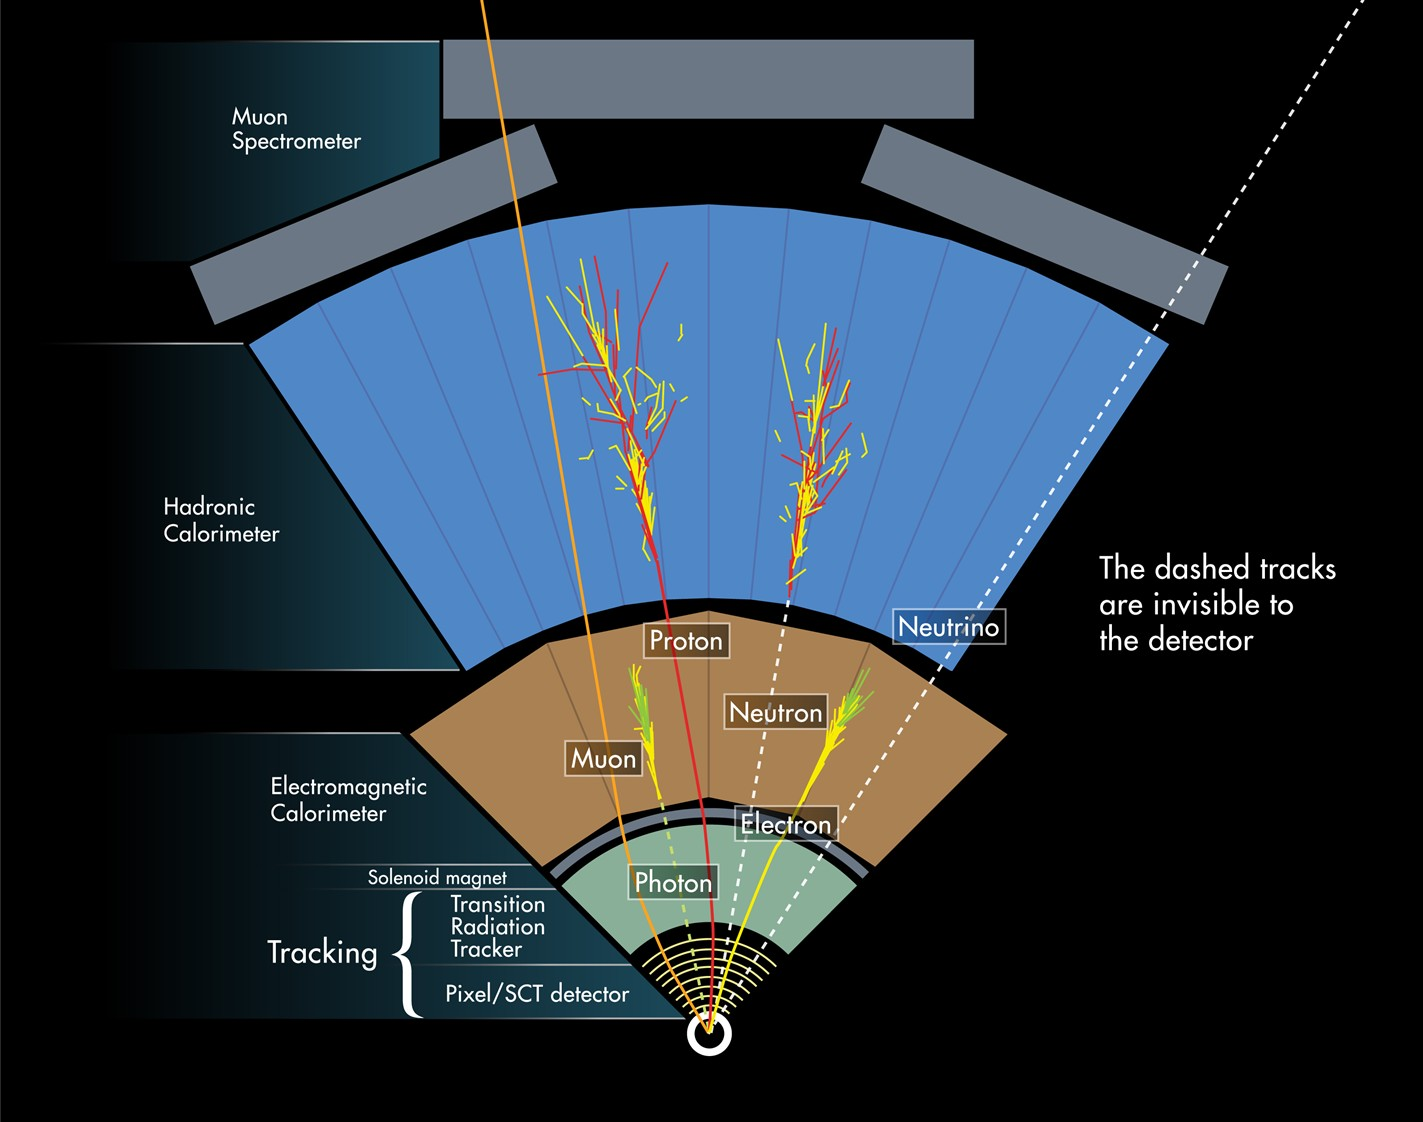
\includegraphics[height=7cm]{reconstruction.jpg}
\end{figure}

\end{frame}

\subsection{Electrons}

\begin{frame}
    \frametitle{Electrons}
\begin{itemize}
    \item A cluster of energy deposits in the EM calorimeter matched
        to a track in the inner detector
    \item Requirements on shower shape, nearby hadronic activity, and
        track-cluster matching reduce backgrounds from non-prompt
        sources (converted photons, light hadrons, and semileptonic
        quark decays)
    \item Calibrated using the $Z$ boson mass peak
\end{itemize}
\vfill
\begin{figure}
\centering
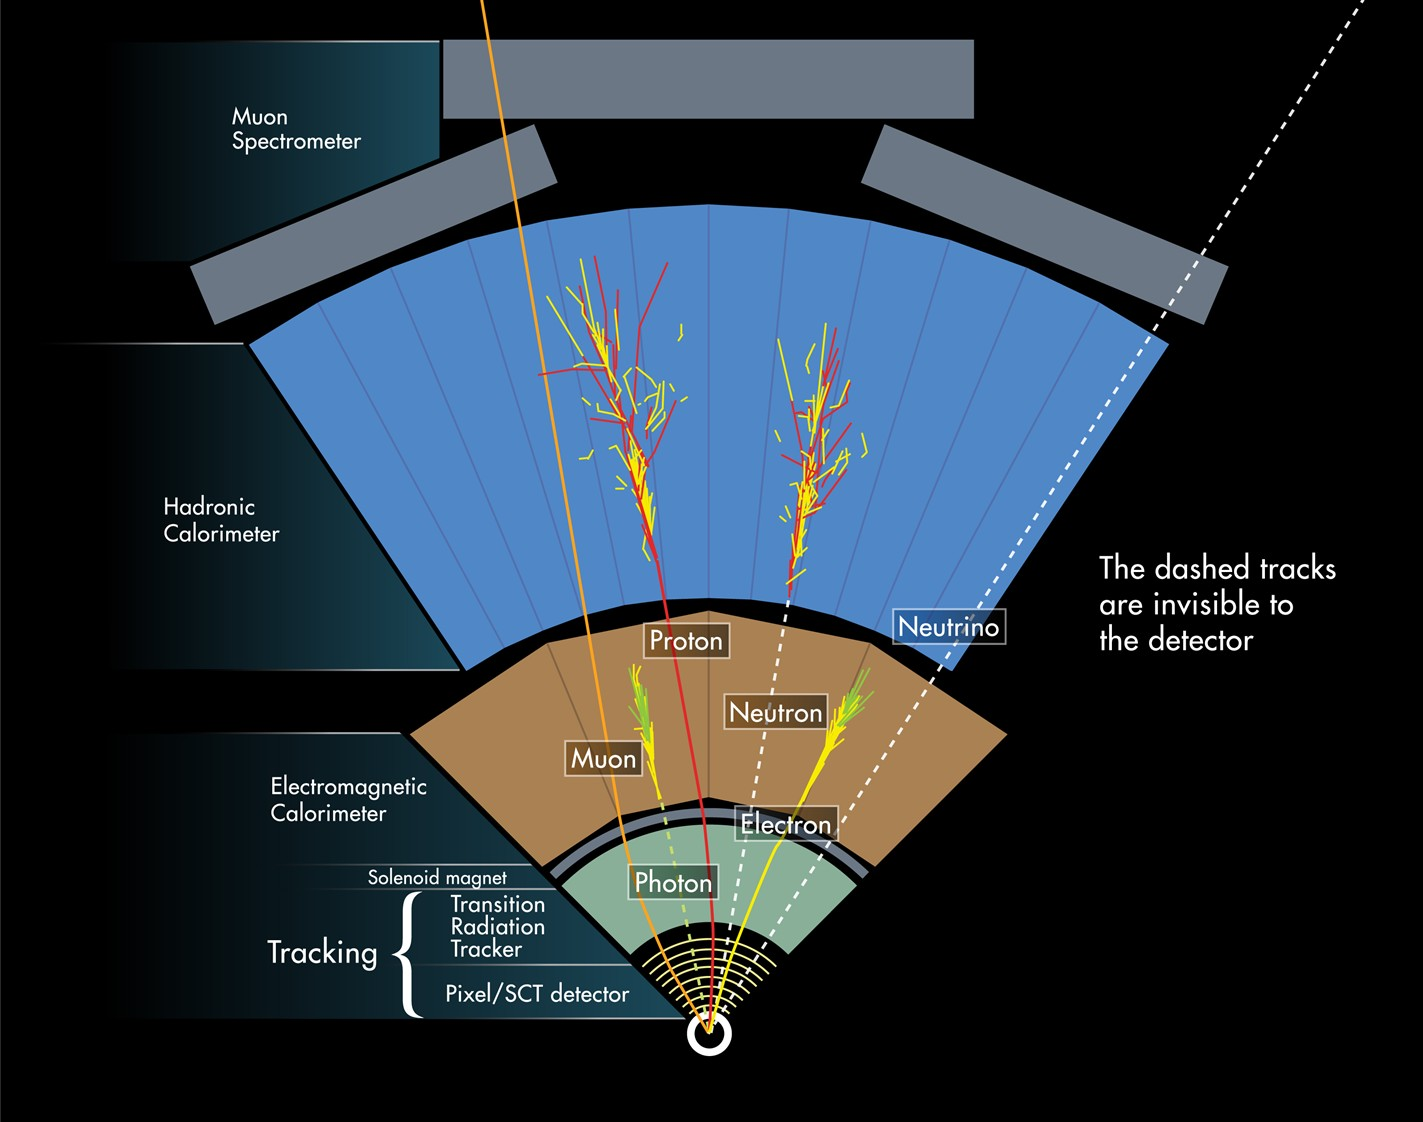
\includegraphics[height=4cm]{reconstruction.jpg}
\end{figure}
\end{frame}

\subsection{Muons}

\begin{frame}
    \frametitle{Muons}
\begin{itemize}
    \item Inner detector track matched to hits in the muon system
    \item Quality requirements on the inner and outer tracks help
        reject mis-reconstructed muons
    \item Isolation from nearby tracks reduces the non-prompt
        background: primarily semileptonic heavy quark decays.
    \item Calibrated using the $Z$ boson mass peak
\end{itemize}
\vfill
\begin{figure}
\centering
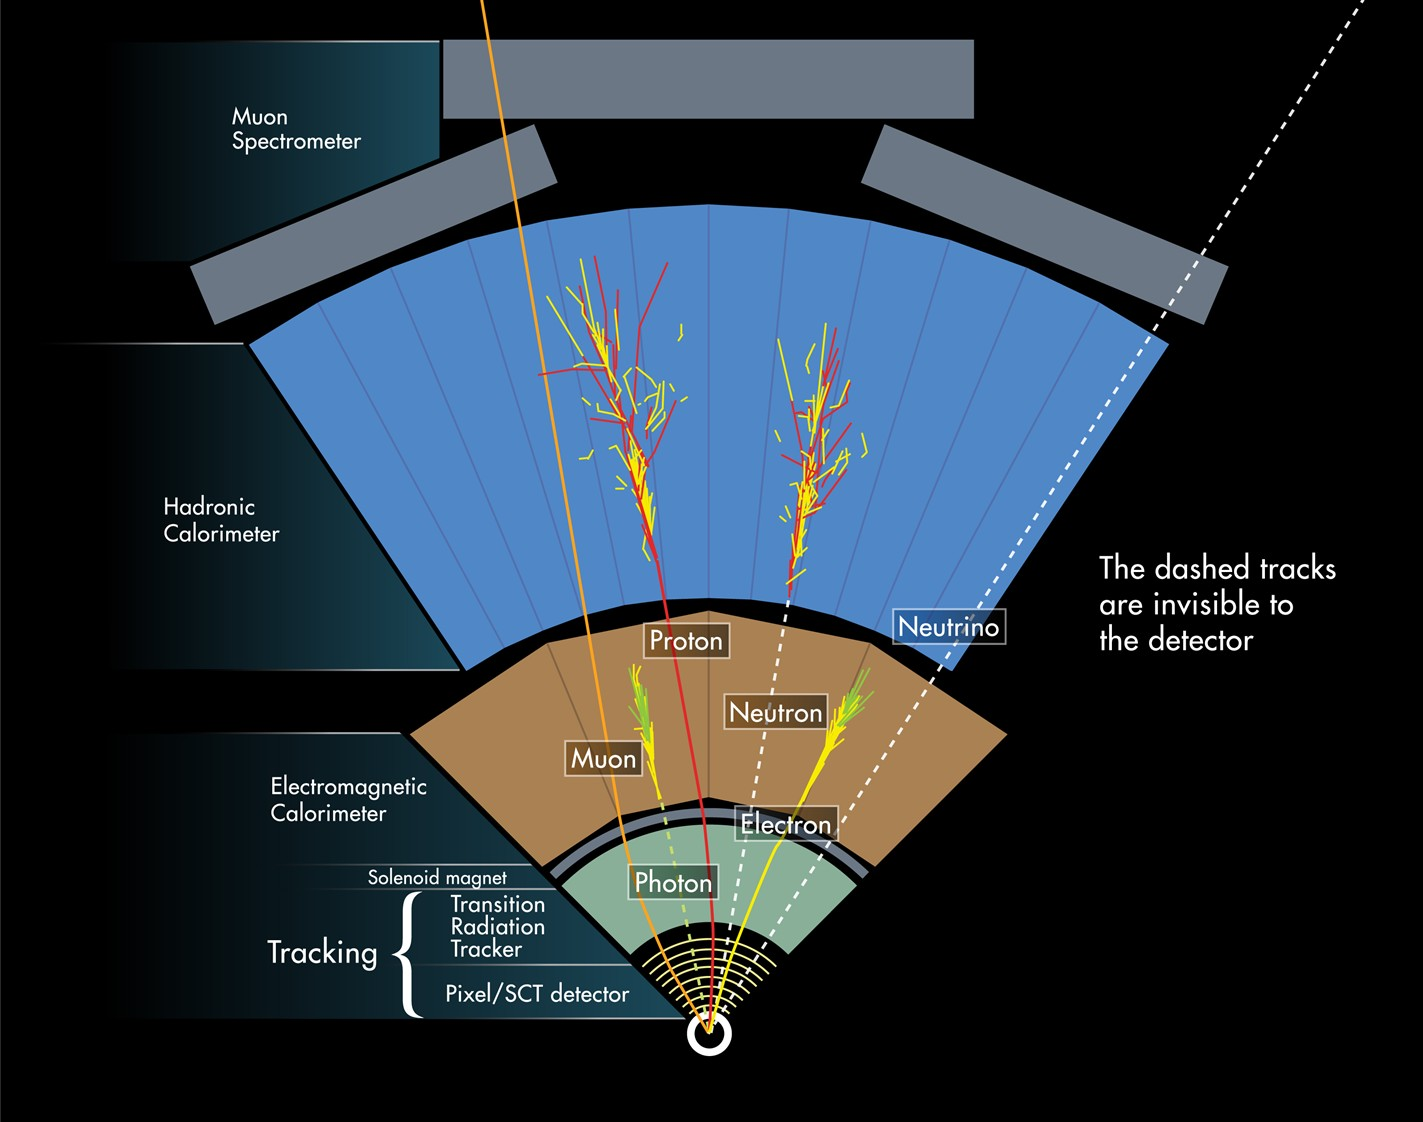
\includegraphics[height=4cm]{reconstruction.jpg}
\end{figure}
\end{frame}

\subsection{Jets}

\begin{frame}[label=jet_reco]
    \frametitle{Jets}
\begin{itemize}
    \item Collection of calorimeter energy deposits used to
        approximate the four-momentum of a quark or gluon
    \item \hlink{jet_clustering}{Clustering algorithms}
        parameterized by an angular distance scale in $\eta-\phi$
        space, $R$ \item Jets calibrated to agree with particle-level
            jets from MC\@.
\end{itemize}
\vfill
\begin{figure}
\centering
    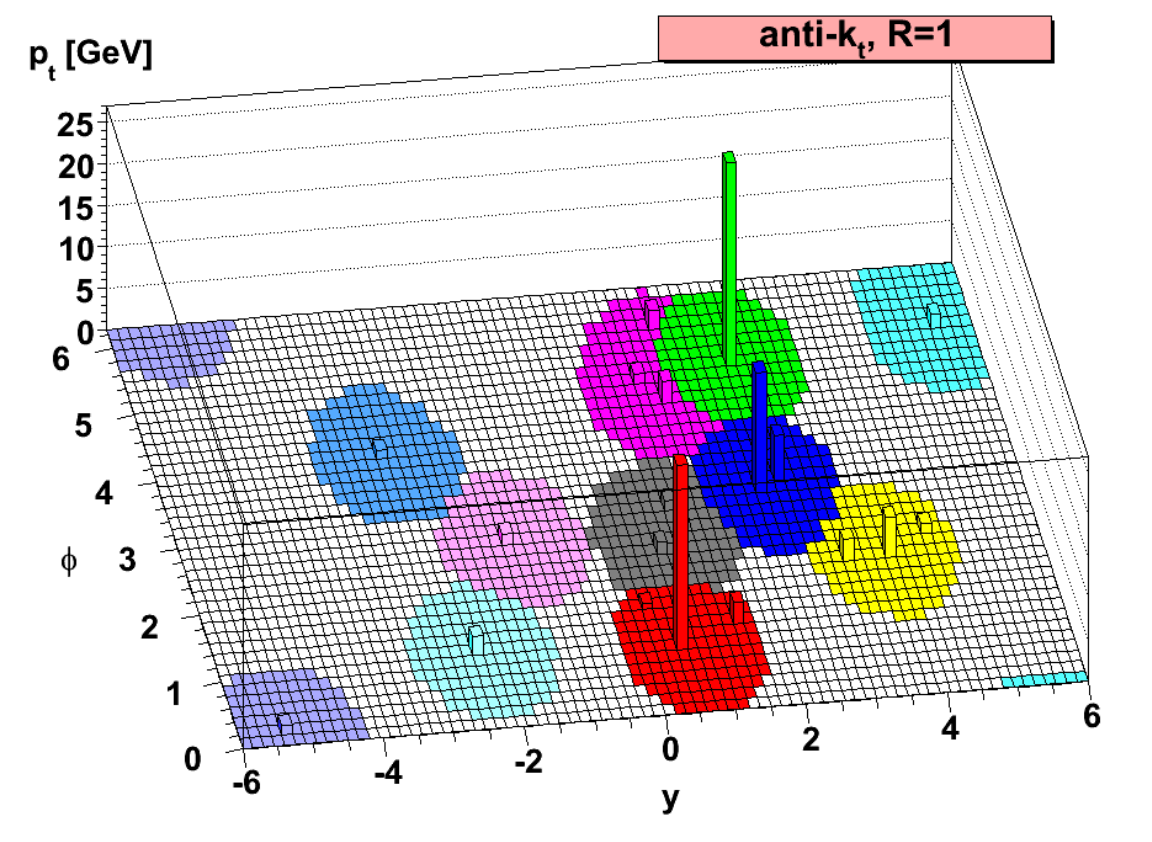
\includegraphics[height=4cm]{akt10.png}
\end{figure}
\end{frame}

\subsection{Missing Transverse Momentum}

\begin{frame}
    \frametitle{\met\ Reconstruction}
\begin{itemize}
    \item Approximates the $p_T$ of particles that do not interact
        with the detector
    \item Defined as the negative vector sum of the transverse momenta
        of all electrons, muons, jets, and other calorimeter deposits
\end{itemize}
\vfill
\begin{figure}
\centering
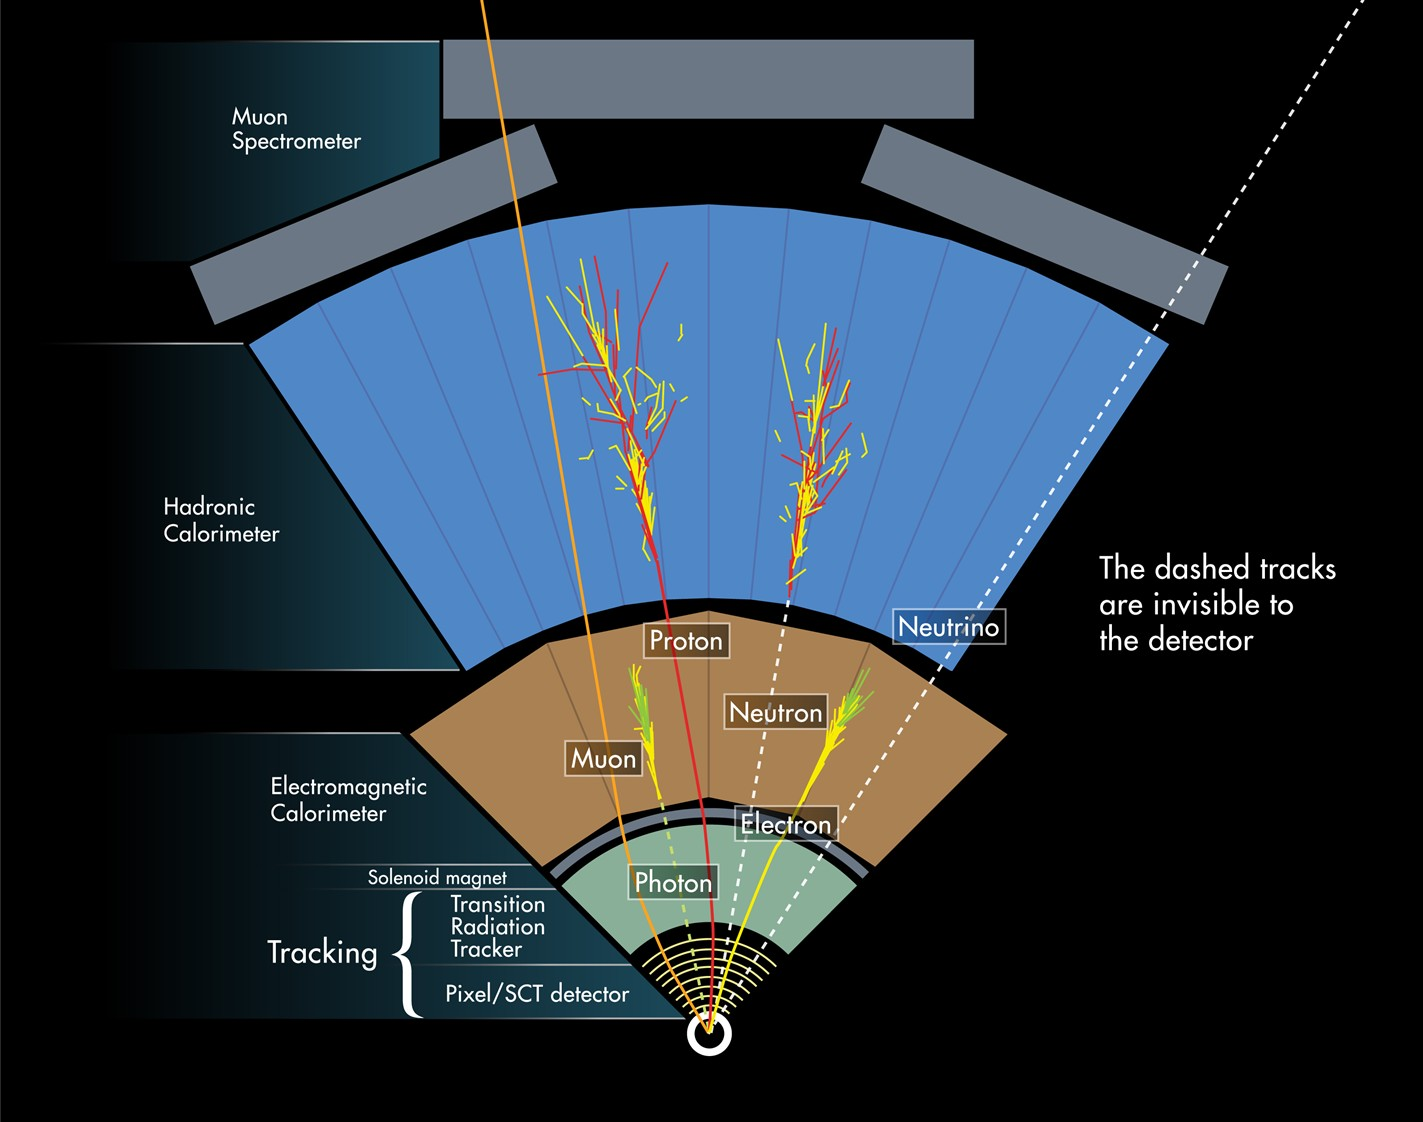
\includegraphics[height=4cm]{reconstruction.jpg}
\end{figure}
\end{frame}
